\documentclass[a4paper,12pt]{report}
\usepackage[a4paper, left=2.5cm, right=2.5cm, top=2.5cm, bottom=2.5cm]{geometry}
\usepackage{graphicx}
\usepackage{geometry}
\usepackage{float}
\usepackage{amsmath}
\usepackage{titlesec} 
\usepackage{lipsum}  
\usepackage{hyperref}
\usepackage{nameref}
\usepackage{xcolor}
\usepackage{etoolbox}
\usepackage{blindtext}
\usepackage{tocloft}
\usepackage{textcomp}
\usepackage{caption}
\graphicspath{{fig/}}






%%%%%%%%%%%%%%%%%%%%%%%%%%%%%%%%%%%%%%%%%%%%This will cause your sections/chapters/subsections to be numbered or not play artound 
\setcounter{secnumdepth}{2}
\setlength{\cftbeforetoctitleskip}{0em}
\setlength{\cftbeforeloftitleskip}{0em}\setlength{\cftbeforelottitleskip}{0em}
%%%%%%%%%%%%%%%%%%%%%%%%%%%%%%%%%%%%%%%%%%%

%%%%%%%%%%%%%%%%%%%%%%%%%%%%%%%%%%%%%%%%%%%
%This simply makes it sotaht there is not a large margin at the top of a new page
%%%%%%%%%%%%%%%%%%%%%%%%%%%%%%%%%%%%%%%%%%%%%%%
\makeatletter
\renewcommand*\@makechapterhead[1]{%
   %\vspace*{50\p@}%
   {\parindent \z@ \raggedright \normalfont
     \ifnum \c@secnumdepth >\m@ne
         \huge\bfseries \@chapapp\space \thechapter
         \par\nobreak
         \vskip 20\p@
     \fi
     \interlinepenalty\@M
     \Huge \bfseries #1\par\nobreak
     \vskip 40\p@
   }}
\renewcommand*\@makeschapterhead[1]{%
   %\vspace*{50\p@}%
   {\parindent \z@ \raggedright
     \normalfont
     \interlinepenalty\@M
     \Huge \bfseries  #1\par\nobreak
     \vskip 40\p@
   }}
\makeatother
%%%%%%%%%%%%%%%%%%%%%%%%%%%%%%%%%%%%%%%%%%%%%%%%%%%%%%%%%%

%%%%%%%%%%%%%%%%%%%%%%%%%%%This makes the list of symbol and abbreviations also have a nice dot fill%%%%%%%%%%%%%%%%%
\makeatletter
\newcommand \Dotfill {\leavevmode \cleaders \hb@xt@ .80em{\hss .\hss }\hfill \kern \z@}
\makeatother
%%%%%%%%%%%%%%%%%%%%%%%%%%%%%%%%%%%%%%%%%%%%%%%%%%%%%%%%

%%%%%%%%%%%%%%%%%%%%renames the title of bibiliography%%%%%%%%%%%%%%%
\renewcommand{\bibname}{References}
%%%%%%%%%%%%%%%%%%%%%%%%%%%%%%%%%%%%%%%%%%%%%%%%%%%%%%%%

%%%%%%%%%%%%%%%%This allows text to be added to the Part heading of documents%%%%%%%%%%%%%%%%%%%%%%%%%%
\makeatletter

\let\LaTeXStandardPart\part%
\newcommand{\unstarredpart@@noopt}[1]{%
  \unstarredpart@@opt[#1]{#1}%
}%

\newcommand{\unstarredpart@@opt}[2][]{%
  \cleardoublepage% (For clearing content before!!!)
  \begingroup%
  \let\newpage\relax%
  \LaTeXStandardPart[#1]{#2}%
  \endgroup%
}%

\newcommand{\starredpart}[1]{%
  \LaTeXStandardPart*{#1}%
}%

\newcommand{\unstarredpart}{%
  \@ifnextchar[{\unstarredpart@@opt}{\unstarredpart@@noopt}%
}%

\renewcommand{\part}{%
  \@ifstar{\starredpart}{\unstarredpart}%
}%
%%%%%%%%%%%%%%%%%%%%%%%%%%%%%%%%%%%%%%%%%%%

%%%%%%%%%%%%%%%%this removes indetation from the first line of a paragraph%%%%%%%%%%%%%%%%%%%%%%
\setlength{\parindent}{0pt}
%%%%%%%%%%%%%%%%%%%%%%%%%%%%%%%%%%%%%%


\begin{document}
\pagenumbering{Roman}
\begin{titlepage}

\begin{center}
\Large\textbf{\\\MakeUppercase{Automated ARM code evaluation
using ARM emulator for Computer
Systems practical assessments}}\par
\end{center}

\Large
\begin{center}
\begin{align*}
&\text{Student Name: } & \text{Mr Michael Alexander Brewis}\\
&\text{Student Number: } & \text{19321023}\\
&\text{Study Leader:} & \text{Dr Arno Barnard}\\
&\text{Date:} & \text{September 2020}
\end{align*}
\end{center}

\begin{figure}[H]
	\begin{center}
	
\includegraphics[scale=0.7]{university.jpg}
	\end{center}	
\end{figure}
\Large

\vfill
\begin{center}
Report submitted in partial fulfilment of the requirements of the module Project (E) 448 for the degree Baccalaureus in Engineering in the Department of Electrical and Electronic Engineering at the University of Stellenbosch
\end{center}	
\end{titlepage}\newpage\cleardoublepage
\chapter*{Acknowledgements}
\label{ack}

I would firstly, like to express my gratitude to Dr Arno Barnard. Without his guidance, considerations and patience, this project would have been impossible. I could not have asked for a better study leader.
\\\\
I would, furthermore, be remiss if I did not thank my friends. Their compassion, motivation and companionship served as a beacon of light, through the long (and often dark) nights comprising the completion of this project. Thank you Jonathan Hendricks for reminding me to stay positive despite the odds. Thank you Mohini Takoorparsadh for your inspirational work ethic and technical assistance. Thank you Andre Bezuidenhoudt, for housing me during the troubled times that 2020 ensured.
\\\\
My gratitude also extends to my bursary givers: G S Fainsinger \& Associates cc. Without the financial support provided, I would not have made it this far.
\\\\
Lastly and most importantly, my unending gratitude extends to my parents. Your unconditional support in this endeavour has resulted in its completion. Thank you for believing in me despite a long chain of failures. Thank you for reminding me that things always turn out fine in the end. Thank you for loving me incomprehensibly.
\begin{figure}[H]
\begin{center}
	
\includegraphics[scale=0.45]{mikePlag.jpg}
\end{center}
\end{figure}

\newpage\cleardoublepage
\section*{Summary}

Currently, there is no system in place to autonomously evaluate student code used in E-Design and Computer System modules. The code is often widely varying, stored in nested repositories and laborious to assess manually. This project aims to alleviate the problem by introducing automation in the form of emulation and code evaluation. 
\\\\
This is done by firstly, investigating possible emulation solutions. High fidelity emulators serve as hardware-independent platforms on which code can be run. By mimicking simple MCU functionality within an emulator, the doors to possible future automation using emulation are left ajar.
\\\\
Once an emulation solution has been achieved, a system whereby student code can autonomously be investigated is warranted. This project will outline the design and implementation of such a system. 

\section*{Opsomming}
Huidiglik is daar geen stelsel in plek om studentekode wat in E-Ontwerp en Rekenaarstelselmodules gebruik word onafhanklik te evalueer nie. Die kode is meestal wisselend, word in beneste bewaarplekke gestoor en is moeisaam om handmatig te assesseer. Hierdie projek se doel is om die bogenoemde probleem te verlig deur outomatisering in te stel in die vorm van emulasie en kode-evaluaring. 
\\\\
Dit word gedoen deur eerstens moontlike emuleringsoplossings te ondersoek. waarHoë-getrouheid emulators dien as platforms wat onafhanklik van hardeware is waarop kode kan loop. Deur die eenvoudige MCU funksionalitiet in ‘n emulator na te boots, kan die moontlikheid van outomatisering wat emulasie benut in die toekoms ondersoek word. 
\\\\
Nadat 'n emulasie oplossing bereik word, kan ‘n stelsel te staan kom waarvolgens studentekode outonomies ondersoek kan word. Hierdie projek sal die ontwerp en implementasie van so ‘n stelsel uiteensit.\newpage\cleardoublepage
\tableofcontents
\newpage\cleardoublepage
\addcontentsline{toc}{chapter}{\listfigurename}
\listoffigures
\newpage\cleardoublepage

\addcontentsline{toc}{chapter}{\listtablename}
\listoftables

\chapter*{List of Symbols}
\label{listSym}
\addcontentsline{toc}{chapter}{List of Symbols}
1.1 $\Omega$ \Dotfill 17

\chapter*{List of Abbreviations}
\label{listAbr}
\addcontentsline{toc}{chapter}{List of Abbreviations}\newpage\cleardoublepage
\pagenumbering{arabic}


\chapter*{1 Introduction}
\label{intro}
\addcontentsline{toc}{chapter}{1 Introduction}

In order to solve the problem as stated in the \color{blue}introduction\color{black}, a solution that allows \hyperref[listAbr]{ARM}-type processors to be mimicked on standard \hyperref[listAbr]{PC} processors is needed. Since most \hyperref[listAbr]{PC}s make use of either intel\textsuperscript{{\tiny{\textregistered}}} or AMD\textsuperscript{{\tiny{\textregistered}}} \hyperref[listAbr]{CPU}'s (which are x86 based architectures - an ubiquitous iteration of \hyperref[listAbr]{CISC}), emulation or simulation is indeed required. This is because, on a machine level, \hyperref[listAbr]{CISC} architecture is incompatible with \hyperref[listAbr]{RISC} assembly language.
It has been established that \hyperref[listAbr]{RISC} architecture will be mimicked on \hyperref[listAbr]{CISC} machines in order to evaluate student code. The degree of mimicry needed depends largely on the application. Whilst emulation mimics a pertaining architecture relatively closely, simulation does so more loosely. Emulation attempts to duplicate one device as accurately as possible in another environment. Simulation, by contrast, is not concerned with low-level duplication of devices, but instead mimics high-level behaviour.\cite{Chris}
In the following chapters, both emulators and simulators will be evaluated as plausible solutions to the problem: \textbf{How can various student generated C and ARM language assembly code, compiled for RISC architectures, be tested on a single x86 (CISC) architecture PCs?} 

\begin{figure}[H]
\begin{center}
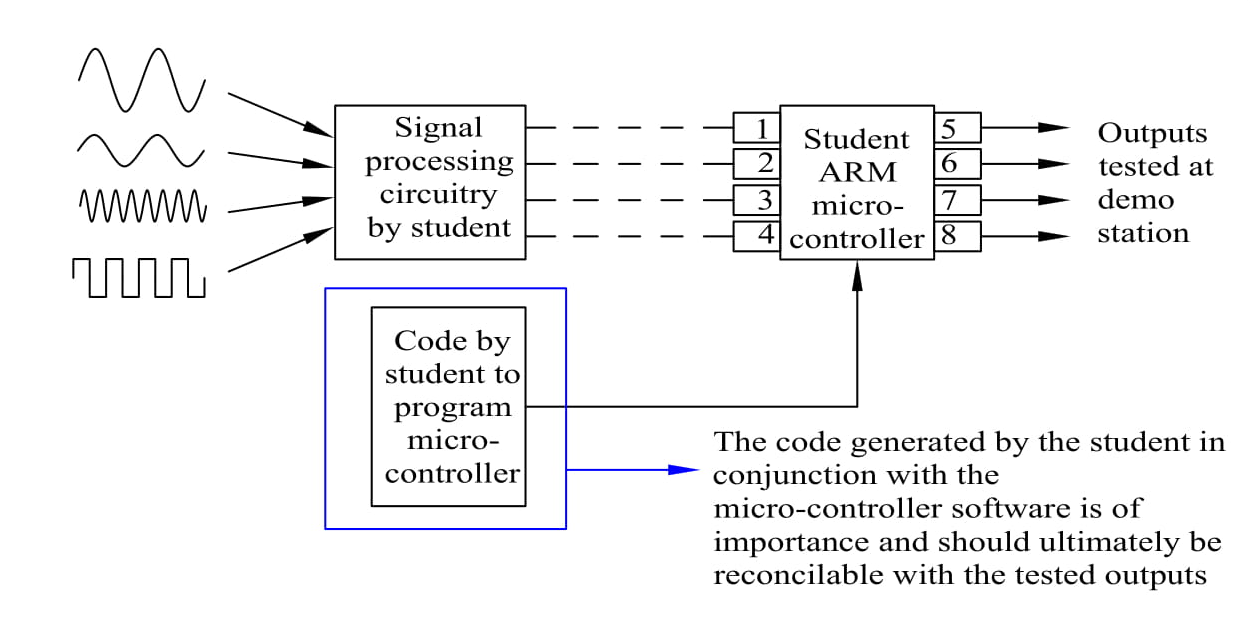
\includegraphics[width = 155mm]{diagram1.png}
\end{center}
\end{figure}
\newpage\cleardoublepage
\part{Emulator Investigation}
\label{part1}
%%\addcontentsline{toc}{chapter}{2 Emulator Investigation}
In order to solve the problem as stated in the \color{blue}introduction\color{black}, a solution that allows \hyperref[listAbr]{ARM}-type processors to be mimicked on standard \hyperref[listAbr]{PC} processors is needed. Since most \hyperref[listAbr]{PC}s make use of either intel\textsuperscript{{\tiny{\textregistered}}} or AMD\textsuperscript{{\tiny{\textregistered}}} \hyperref[listAbr]{CPU}'s (which are x86 based architectures - an ubiquitous iteration of \hyperref[listAbr]{CISC}), emulation or simulation is indeed required. This is because, on a machine level, \hyperref[listAbr]{CISC} architecture is incompatible with \hyperref[listAbr]{RISC} assembly language.
\\\\
It has been established that \hyperref[listAbr]{RISC} architecture will be mimicked on \hyperref[listAbr]{CISC} machines in order to evaluate student code. The degree of mimicry needed depends largely on the application. Whilst emulation mimics a pertaining architecture relatively closely, simulation does so more loosely. Emulation (and subsequently emulators) attempts to duplicate one device as accurately as possible in another environment. Simulation, by contrast, is not concerned with low-level duplication of devices, but instead mimics high-level behaviour. \cite{Chris}
\\\\
For the evaluation of student specific code, a simulator will suffice as low-level architecture need not be 

\part{High Level Code Structure Evaluation and Comparison}
\label{part2}
Here I am simply putting this to test a git push. \cite{Hashim}


\part{High Level Code Structure Testing}
\label{part3}
%%\addcontentsline{toc}{chapter}{2 Emulator Investigation}



\part{Conclusion}
\label{conc}

\chapter*{}
\label{bib}
\addcontentsline{toc}{chapter}{References}

\bibliography{bib/thesis.bib}
\bibliographystyle{ieeetr}
\chapter*{Appendix A: Project planning schedule}
\label{A}
\addcontentsline{toc}{chapter}{Appendix A: Project planning schedule}


\chapter*{Appendix B: Outcomes compliance}
\label{B}
\addcontentsline{toc}{chapter}{Appendix B: Outcomes compliance}
\chapter*{Appendix C}
\label{C}
\addcontentsline{toc}{chapter}{Appendix C}
\end{document}

